\documentclass[11pt]{article}
\usepackage{bm}
\usepackage[margin=1.7cm,top=2.5cm,bottom=2.5cm,letterpaper]{geometry}
%\usepackage{enumitem}
\usepackage{tikz}%,graphicx,wrapfig}
\usepackage{amsmath}
\usepackage{mathpazo}
%\usepackage{pgfplots}
%\usepackage{times}
%\usepackage[document]{ragged2e}
%\usepackage[none]{hyphenat}
\usepackage{siunitx}
%\usepackage{multicol}
\usepackage{fancyhdr}

\usetikzlibrary{decorations.pathmorphing,patterns}

\newcommand{\mb}[1]{\mathbf{#1}}
%\newcommand{\iii}{\bm{\hat{\imath}}}
%\newcommand{\jjj}{\bm{\hat{\jmath}}}
\newcommand{\pic}[2]{\includegraphics[width=#1\textwidth]{#2}}

\setlength{\parskip}{15pt}

\sisetup{
  detect-all,
  %number-math-rm=\mathnormal,
  %  text-sf=\sffamily,
  %  text-rm=\sffamily,
  inter-unit-product =\ensuremath{\cdot{}},
  per-mode=symbol,
  group-separator={,},
}

\title{Rigid-Body Rotational Motion}
\author{Timothy M.\ Leung, Ph.D.}
\date{\today}

\pagestyle{fancy}
\chead{}
\lhead{Olympiads School}
\rhead{Advanced Placement Physics}
\lfoot{Solutions to Free Response Questions}
\cfoot{-\thepage-}
\rfoot{}


\begin{document}

\maketitle

\section{Pure Rolling of Rigid Body on Flat Surface}
The case of the rolling ball is a standard example of combining the dynamics of
translational and rotational motions of a rigid body. In this example, a
perfectly smooth ball rolls on a perfectly smooth surface without slipping
(rolling without slippage is called \textbf{pure rolling}). The force diagram
is shown in Fig.~\ref{roll-flat}. Notice that \emph{there is no friction between
  the ball and the surface}. In theory, the steel ball bearing should be able
to roll along the surface forever, as there is neither a net force nor a net
torque acting on the ball.
\begin{figure}[!ht]
  \centering
  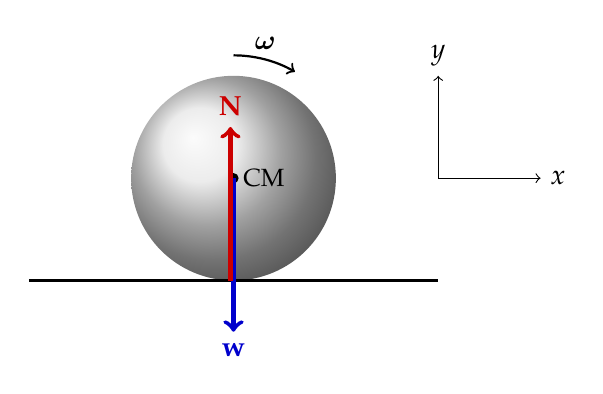
\begin{tikzpicture}[scale=1.3]
    \tikzstyle{balloon}=[ball color=gray!20];
    \shade[balloon](0,0) circle(1);
    \draw[thick](-2,-1)--(2,-1);
    \draw[thick,->](0,1.2) arc(90:60:1.2) node[midway,above]{$\bm{\omega}$};
    \draw[->](2,0)--(3,0) node[pos=1,right]{$x$};
    \draw[->](2,0)--(2,1) node[pos=1,above]{$y$};
    \fill(0,0) circle(.05) node[right]{\small CM};
    \draw[->,ultra thick,blue!80!black](0,0)--(0,-1.5)
    node[pos=1,below]{$\mb{w}$};
    \draw[->,ultra thick,red!80!black](-.03,-1)--(-.03,.5)
    node[pos=1,above]{$\mb{N}$};
  \end{tikzpicture}
  \caption{Force diagram on a steel ball bearing rolling on a smooth flat
    surface without slipping.}
  \label{roll-flat}
\end{figure}

But any casual observer will notice that the steel ball will, in reality, slow
down and eventually stop. So what is causing this?

Firstly, we should recognize neither the ball bearing nor the rail are
perfectly smooth. When the ball rolls over a bump, the surface roughness means
that the normal force does not necessarily points towards the centre of the
ball. This means that unlike in Fig. A, there is a net force and net torque
that will slow down the motion of the ball.

%Figure B: Free-body diagram of a ball bearing rolling over a bump.
%
Secondly, we should recognize that there is no such thing as a perfectly rigid
body. Both the ball and the surface deform as they make contact. A perfect
illustration is how a tire flattens when it makes contact with the ground.

%, instead of a steel ball bearing, we have a wheel with a rubber tire. In this case, the slowing down also comes from the rolling resistance from deformation of the tire as it makes contact with the ground.
%
%
\section{Pure Rolling on an Inclined Surface}
But what if the ball rolls without slippage down a ramp instead? The free-body
diagram for a ball rolling down a ramp of angle $\theta$ is shown in
Fig.~\ref{roll-ramp}. This time, there is a static friction $\mb{f}_s$ acting
up the ramp.
\begin{figure}[!ht]
  \centering
  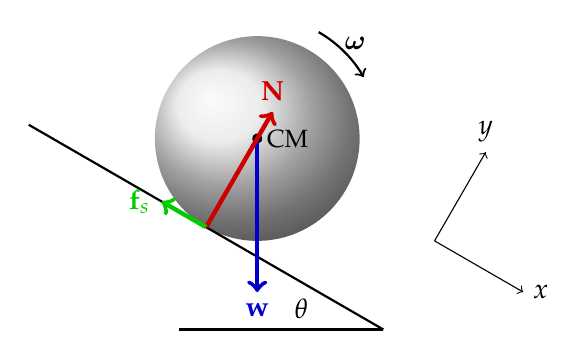
\begin{tikzpicture}[scale=1.3]
    \begin{scope}[rotate=-30]
      \tikzstyle{balloon}=[ball color=gray!20];
      \shade[balloon](0,0) circle(1);
      \draw[thick](-2,-1)--(2,-1);
      \draw[thick,->](0,1.2) arc(90:60:1.2) node[pos=.3,right]{$\bm{\omega}$};
      \draw[->](2,0)--(3,0) node[pos=1,right]{$x$};
      \draw[->](2,0)--(2,1) node[pos=1,above]{$y$};
      \fill(0,0) circle(.05) node[right]{\small CM};
      \draw[->,ultra thick,blue!80!black,rotate=30](0,0)--(0,-1.5)
      node[pos=1,below]{$\mb{w}$};
      \draw[->,ultra thick,red!80!black](.0,-1)--(.0,.3)
      node[pos=1,above]{$\mb{N}$};
      \draw[->,ultra thick,green!80!black](.0,-1)--(-.5,-1)
      node[pos=1,left]{$\mb{f}_s$};
      \begin{scope}[rotate around={30:(2,-1)}]
        \draw[thick](2,-1)--(0,-1) node[pos=.4,above]{$\theta$};
      \end{scope}
    \end{scope}
  \end{tikzpicture}
  \caption{Force diagram on a steel ball bearing rolling on a smooth ramp
    without slipping. The ball travels distance $d$ to the bottom of the ramp.}
  \label{roll-ramp}
\end{figure}
The weight of the ball acts at the centre of gravity, while the normal force
acts at the point of contact. Neither forces generate any torque about the CM,
therefore, without
friction, the ball will just \emph{slide} down the ramp without any rotation.
To solve this problem, we have three dynamic equations along the three axes:
\begin{align}
  \sum F_x&=mg\sin\theta-f_s=ma\\ \label{f_x}
  \sum F_y&=N-mg\cos\theta=0\\
  \sum\tau&=rf_s=I_z\alpha \label{tau}
\end{align}
At this stage, the actual static friction force is not known and is a quantity
that needs to be solved. Knowledge of the coefficient of static friction
$\mu_s$ may not be useful, because it only tells you the \emph{maximum} static
friction force, not the actual fritcion force that exists. However, we will use
it to double check to see if the answer makes sense.

Inserting the expression for the moment of inertia of the ball\footnote{Note
  that if instead of using a solid ball, we will have to use the moment of
  inertia of
  those objects:\\
  Hollow sphere\\
  Solid cylinder\\
  Hollow cylinder} and recognizing that for pure rolling,
$\displaystyle\alpha=\frac{a}{r}$, we can use Eq.~\ref{tau} to express static
friction in terms of $a$:
\begin{equation}
  f_s=\frac{I_z\alpha}{r}=
  \label{f_s}
\end{equation}
Substituting the expression in Eq.~\ref{f_s} into Eq.~\ref{f_x}, the force
equation in the $x$-direction becomes:
\begin{equation}
  mg\sin\theta-f_s=ma
\end{equation}
Cancelling the mass terms and solving for acceleration, we find a value of:
\begin{equation}
  a=
  \label{pure-roll-accel}
\end{equation}
As weight, normal force and friction are all time independent, acceleration is
constant.

Compare the results in Eq.~\ref{pure-roll-accel} to that of an object sliding
without friction down the same ramp, the acceleration for the sliding block is
$a=g\sin\theta$ which is higher than the pure rolling case. The simplest
explanation is that some of the gravitational potential energy is converted to
both translational and rotational kinetic energies, while for the sliding case,
all of the potential energy is converted into translational kinetic energy.

There is, of course, one check that we must make, that is to make sure that the
friction calculated in Eq.~\ref{f_s} has not exceeded the maximum static
friction, given by
\begin{equation}
  \max f_s=\mu_s N
\end{equation}
If this is indeed the case, it means that the ball will actually slip while
rolling down the ramp, and the friction at the contact point is in fact kinetic
friction.

Since acceleration is constant, we can use the basic kinematic equation to
compute the speed of the ball when it reaches the bottom of the ramp, a
distance $d$ away. For simplicity, we assume that the ball starts from rest:
\begin{equation}
  v=\sqrt{2ad}=
\end{equation}
Of course, there is a much simpler way to find $v$, that is, by using the
conservation of energy.
\begin{align*}
  \Delta U_g&=K_t+K_r\\
  mg\textcolor{red}{\Delta h}&=\frac12 mv^2+
  \frac12
  \textcolor{blue}{I}\textcolor{orange}{\omega}^2\\
  mg\textcolor{red}{d\sin\theta}&=\frac12 mv^2+\frac12
  \left(\textcolor{blue}{\frac23 mr^2}\right)
  \left(\textcolor{orange}{\frac{v}{r}}\right)^2\\
  &=\frac23mv^2
\end{align*}
Now cancelling mass terms on both sides, and solving for $v$, we arrive at the
same expression as using dynamics and kinematics equations:


This is pretty significant for the novice leave because while there is indeed
friction, this friction didn't do any work. This should not be a surprise,
because in order for a force to do any work, it has to actually \emph{move}
something. This is clearly not the case if friction is \emph{static}. To be
clear, if the ball slips, then there is definitely work done by kinetic
friction.
%
%Alright, so it slips on a flat surface
%
%The net force comes from the kinetic friction, which accelerates the ball towards the right. This same friction force also generates a bit torque in the counter clockwise direction, slowing down the rotation.
%
%\fbox{
%  \begin{minipage}{.97\linewidth}
%    \textbf{Free Response Question 4:} A steel ball is dropped from a point with
%    $(x,y)$ coordinate of $(\SI{8}{\metre},\SI{16}{\metre})$. At the same time,
%    another ball is launched from the origin with a speed of
%    \SI{20}{\metre\per\second} at an angle of \ang{30}.
%    \begin{enumerate}[noitemsep,topsep=0pt]
%    \item Find the minimum distance of separation occur of the two balls.
%    \item At what time does this separation occur?
%    \item Give the coordinates of the two balls for the minimum separation.
%    \end{enumerate}
%  \end{minipage}
%}
%
%There are two ways to solve the problem. The first method \emph{looks} easy on
%first glance, but will require a lot of calculus. The second method, on the
%other hand, is a straightforward geometry problem that requires a bit of
%ingenuity.
%
%\textbf{\underline{Method 1 (not recommended)}}
%
%The most straightforward approach is to express the distance between the steel
%balls as a function of time, and then take the derivative with respect to time
%to find out when it occurs $t$ and minimum value of $d$.
%
%Let's call the steel ball being dropped $A$, and the ball that is launched
%$B$. Their respective position in the coordinate system are expressed as
%functions of time using kinematic equations\footnote{For the $x$ direction,
%  $x=v_xt$ and for the $y$ direction, $y=y_0+v_{y0}t-\frac12gt^2$.}, and using
%$g=\SI{10}{\metre\per\second^2}$ for both cases\footnote{which is acceptable
%  for all AP exams} for simplicity.
%\begin{align}
%  \mb{x}_A &= 8\iii + (16-5t^2)\jjj \\
%  \mb{x}_B &=20\cos\ang{30}t\iii+(20\sin\ang{30}t-5t^2)\jjj
%\end{align}
%The ``displacement'' vector between $A$ and $B$ can be expressed as:
%\begin{equation}
%  \Delta\mb{x}
%  =\mb{x}_A-\mb{x}_B
%  =(8-20\cos\ang{30}t)\iii + (16-20\sin\ang{30}t)\jjj
%  \label{no-g}
%\end{equation}
%Not surprisingly, the gravitational acceleration term $\frac12gt^2=5t^2$ term
%cancels, because both $A$ and $B$ are free-falling objects with the same
%downward acceleration. The square of the \emph{distance} between $A$ and $B$ are
%expressed as:
%\begin{equation}
%  d^2 =(8-20\cos\ang{30}t)^2 + (16-20\sin\ang{30}t)^2
%\end{equation}
%What we will need to do now is to take the time derivative of $d^2$ with
%respect to time, and to find $d$ and $t$. This process is laborious and
%tedious (and prone to error for someone uncomfortable with using chain rule)
%and therefore generally not recommended. We will instead try a completely
%different approach.
%
%\textbf{\underline{Method 2}}
%
%However, we have already noted that in Equation~\ref{no-g}, acceleration due to
%gravity terms cancel, which means that the minimum separation distance $d$ does
%not depend on $g$! We instead consider an observer who is falling alongside
%steel ball $A$ (which is equivalent to effectively treating $g=0$.) In this
%case, the observer sees that $A$ remains stationary while $B$ travels in a
%straight line instead of the parabolic path of a projectile. The observer's
%point of view is shown in Fig.~\ref{falling}. The minimum distance of
%separation occurs at $C$ in this frame of reference, with a value of $d$.
%\begin{figure}[ht]
%  \begin{center}
%    \begin{tikzpicture}[scale=.4]
%      \draw[->](0,0)--(17,0) node[pos=1,right]{$x$};
%      \draw[->](0,0)--(0,17) node[pos=1,above]{$y$};
%      \fill(8,16) circle(.18) node[above]{$A$};
%      \fill(8,4.62) circle(.1) node[above left]{$E$};
%      \fill(8,0) circle(.1) node[below]{$D$};
%      \draw[dashed](8,16)--(8,0);
%      \draw[dashed](12.9,7.46)--(12.9,0) node[below]{$C'$};
%      \draw[->](3,0) arc(0:30:3) node[midway,right]{\ang{30}};
%      \draw[->](8,13) arc(270:300:3) node[midway,below]{\ang{30}};
%      \begin{scope}[rotate=30]
%        \draw[very thick](0,0)--(18,0);
%        \fill(18,0) circle(.18) node[right]{$B$};
%      \end{scope}
%      \draw[dashed](8,16)--(12.9,7.46) node[midway,above right]{$d$};
%      \fill(12.9,7.46) circle(.1) node[below right]{$C$};
%    \end{tikzpicture}
%  \end{center}
%  \caption{Observing the steel balls while free-falling}
%  \label{falling}
%\end{figure}
% Using basic geometry, we can find distance $DE$ and $AE$:
% \begin{align*}
%   DE&=8\tan\ang{30}=\SI{4.6}{\metre}\\
%   AE&=16-DE=\SI{11.4}{\metre}
% \end{align*}
%Using basic trigonometry again, we can now find the minimum distance of
%separation:
%\begin{displaymath}
%  d=AE\cos\ang{30}=\boxed{\SI{9.9}{\metre}}
%\end{displaymath}
%The second part is slightly trickier, because we have (so far) ignored
%acceleration due to gravity. However, there is no acceleration in the $x$
%direction, i.e.\ the horizontal distance that $B$ travels is the same. We
%need to compute $DC'$ which is just
%\begin{displaymath}
%  DC'=d\sin\ang{30}=\SI{4.9}{\metre}
%\end{displaymath}
%which means that in the time to reach minimum separation distance, the steel
%ball $B$ has travelled $8+4.9=\SI{12.9}{\metre}$ horizontally. We can now use
%the kinematic equation in the $x$-direction to compute $t$:
%\begin{displaymath}
%  t=\frac{\Delta x}{v_x}=\frac{12.9}{20\cos\ang{30}}=\boxed{\SI{.75}{\second}}
%\end{displaymath}
%Finally, we substitute $t$ back into the \emph{actual} position of $A$ and $B$
%to compute their \emph{actual} location when the minimum separation occurs:
%\begin{align*}
%  \mb{x}_A &= 8\iii + (16-5t^2)\jjj = \boxed{8\iii+13.2\jjj} \\
%  \mb{x}_B &=20\cos\ang{30}t\iii+(20\sin\ang{30}t-5t^2) \jjj
%  =\boxed{12.9\iii+1.7\jjj}
%\end{align*}
%\newpage
%
%\fbox{
%  \begin{minipage}{.97\linewidth}
%    \textbf{Free Response Question 6:} A trail bike take off from a ramp with
%    velocity $\mb{v}_0$ at angle $\theta$ to clear a ditch of width $x$ and
%    land on the other side, which is elevated at a height $H$.
%    \begin{center}
%      \pic{.4}{../homework/trail-bike.jpg}
%    \end{center}
%    \begin{enumerate}[noitemsep,topsep=0pt]
%    \item For a given angle $\theta$ and distance $x$, what is the upper limit
%      for $H$ such that the bike has an chance of making the jump?
%    \item For $H$ less than this upper limit, what is the minimum take-off speed
%      $v_0$ necessary for a successful jump?
%    \end{enumerate}
%    Neglect the size of the trail bike, and assume that covering a horizontal
%    distance $x$ and a vertical distance $H$ is sufficient to clear the ditch.
%  \end{minipage}
%}
%
%To solve this problem, we must break down the initial velocity $\mb{v}_0$ into
%its horizontal ($\iii$) and vertical ($\jjj$) directions, i.e.:
%\begin{displaymath}
%  \mb{v}_0=v_o\cos\theta\iii+v_0\sin\theta\jjj
%\end{displaymath}
%Ignoring air resistance, the only acceleration will be due to gravity (which is
%constant), in the $\jjj$ direction. Also assuming that $H$ is the maximum
%height that the dirt bike reaches. We can use the kinematic equations to obtain
%an expression for $H$ in terms of $v_0$ and $\theta$:
%\begin{equation}
%  v_y^2=v_{y0}^2-2gH\quad\longrightarrow\quad
%  0=v_o^2\sin^2\theta-2gH\quad\longrightarrow\quad
%  \boxed{H=\frac{v_o^2\sin^2\theta}{2g}}
%  \label{HH}
%\end{equation}
%Note that this is the same calculation we used to obtain the maximum height
%for a symmetric trajectory projectile motion. The time it takes to reach this
%height is also straightforward to obtain:
%\begin{equation}
%  v_y=v_{y0}-gt\quad\longrightarrow\quad
%  0=v_0\sin\theta-gt\quad\longrightarrow\quad
%  \boxed{t=\frac{v_0\sin\theta}{g}}
%\end{equation}
%Likewise, this hte exactly \emph{half} of the value for a symmetric projectile.
%In the $\iii$ direction, there is no acceleration, and the width of the ditch
%$x$ can be related to the initial velocity as:
%\begin{equation}
%  x=v_xt=v_0\cos\theta\left(\frac{v_0\sin\theta}{g}\right)
%  =\boxed{\frac{v_0^2\sin\theta\cos\theta}{g}}
%  \label{halfrange}
%\end{equation}
%For completeness, Eq.~\ref{halfrange} is also \emph{half} the range of a
%symmetric projectile. Substituting the expression for $H$ from Eq.~\ref{HH}
%into Eq.~\ref{halfrange}, and solving for $H$ obtains the answer to the first
%part of the question:
%\begin{equation}
%  x=\frac{2H\cos\theta}{\sin\theta}
%  \quad\longrightarrow\quad
%  \boxed{H=\frac12x\tan\theta}
%  \label{solution1}
%\end{equation}
%For the second part of the question, we assume that the width of the ditch
%$x$ and the angle of the ramp $\theta$ are constant, and that $H$ is the only
%thing that will change. Therefore, we want to express $v_0$ needed to clear $H$
%in terms of $x$ and $\theta$. Then any $v_0$ less than this value will clear a
%height less than $H$. Equating the expression for $H$ in Eq.~\ref{solution1} to
%Eq.~\ref{HH}, and rearranging terms:
%\begin{align}
%  \frac{v_0^2\sin^2\theta}{2g}&=\frac12x\tan\theta
%  =\frac12 x\frac{\sin\theta}{\cos\theta}\\
%  v_0^2&=\frac{gx}{\sin\theta\cos\theta}=\frac{2gx}{\sin(2\theta)}
%\end{align}
%Finally, solving for $v_0$ we have the expression for the velocity to clear
%\begin{equation}
%  \boxed{v_0\geq\sqrt{\frac{2gx}{\sin(2\theta)}}}
%\end{equation}
\end{document}
